\chapter{System Design}

The complete work presented here can be divided into several parts right from
taking in a topic as input, finding out relevant documents, tagging words as
probable answer words, and eventually generating questions from it. 

\begin{figure}
	\caption{Architecture of Model}
	\centering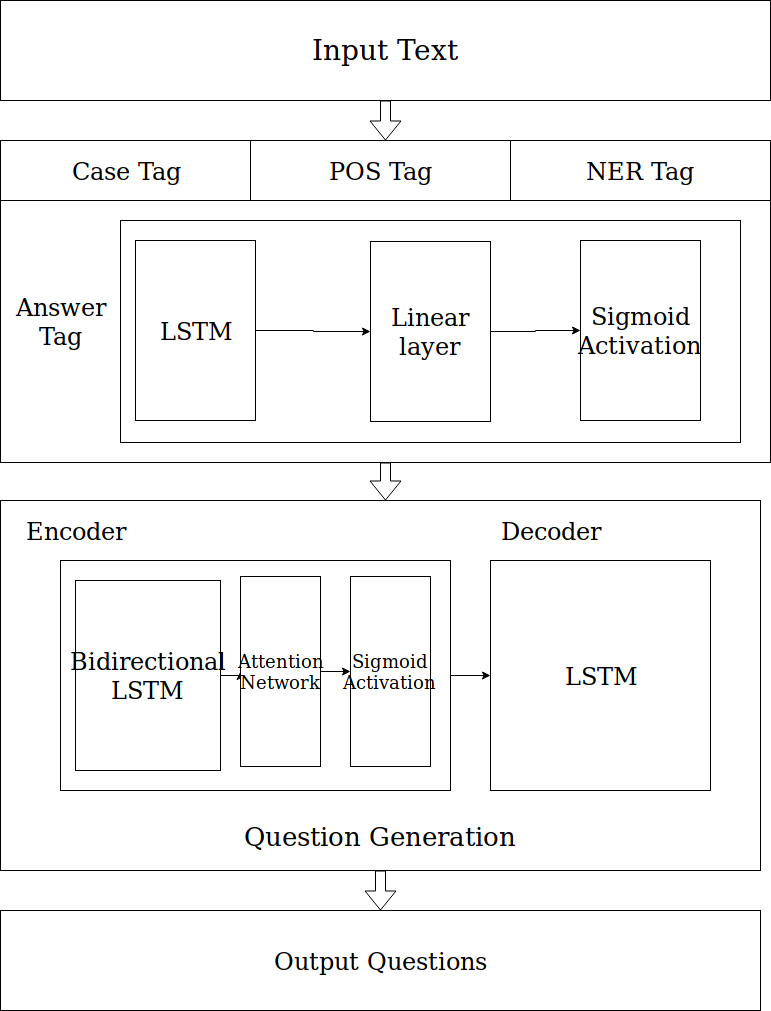
\includegraphics[width=10cm]{5.png}
\end{figure}

\section{Topic Input \& Data gathering}

Initially, the user shall enter his/her topic of interest into the software. The
software shall then crawl the web and gather links to various web pages relevant
to the topic given by the user. On getting the links, further the software shall
scrape those links and parse the HTML pages to get the information content in
those web pages.  

However, all the content received can be classified into three parts. The first
part consists of markup language tasks and syntax, the second part shall contain
data unrelated to the topic of interest, and the third shall be the data which
is useful and relevant both to the topic of interest. The data classified into
the first part, is removed by searching for markup language tasks in the
obtained data.  On finding such tags, the lines containing such tags shall be
eliminated from the useful data text. For identifying data in the second part,
the semantic meaning of the words and the web page from where the data has been
input is taken into consideration. Thus eventually the system has data which can
be used for generating questions on the users topic of interest.


\section{Pre processing block}

The processing done at this stage can be broken down into 4 independent tasks.
The output of each of these four tasks work as features for the question
generation algorithm. The four tasks and their work can be summarized as follows
-

\begin{enumerate}

\item Case of the word in context - This feature determines whether the first
letter of the word is in lower or upper case. The output of this case thus
determines whether the word is the starting word of the context. In quite a few
cases, the starting word of the context dominates in meaning, and hence has been
considered as a feature in the problem.

\item NER Tagging - The 7 set Stanford NER Tagging is used in the system. The
NER Tagging helps in finding out a type of a noun the word is, like a place, a
date or a person. As per the tag different Wh questions are created and hence
the feature is of great significance in the problem.

\item POS Tagging - POS tags are important in generating patterns based on their
frequency in the contexts. Frequently occuring series of consecutive POS tags
that form answer words in the training sentences are most probable to be the
best sources for generating questions in test contexts as well.

\item Answer Words - This feature is the most important of all the four
features. This feature talks of whether the word in consideration is an answer
word or not, in the question to be formed. Only those words that are answer
words are given paramount importance in the question generating process.

\end{enumerate}

So to achieve this goal, a simple model containing a lstm and linear layer is
created. The output of the model is binary string which is 1 for the Answer Tag
and 0 elsewhere.  The LSTM help in remembering the previous answer tags thus
helping in predicting the current tag.

\section{Question Generation - Algorithm}

\begin{itemize}

	\item \textbf{Context Reader and Encoder}

Context reader is a bi-directional long short-term memory (bi-LSTM) network with
		600 hidden layers. Bi-LSTM processes the input words in both the
		forward and backward direction. Encoder creates context word
		vectors from the preprocessed input provided.

\item \textbf{Decoder and Softmax activation}

	The question-generator generates a question word one-by-one by following
		two internal calculations. The unidirectional LSTM in the
		decoder maps the current question word with fixed-sized vector,
		which is the hidden state of the network. Then the second
		calculation, i.e. the softmax function calculates the
		probability distribution over all words from a fixed question
		vocabulary.

\item \textbf{Relevance of Question}

	To select the relevant question, pointer network is used. Pointer
		network calculates the output word probabilities as a mixture of
		two probabilities, one over the question vocabulary and the
		other over the input context vocabulary

\end{itemize}

\section{Output}

In the end, the system shall generate questions on either the topic of interest
specified to the user or the text given as input to the system. The system can
generate three types of questions. The first type is Fill in The Blank
questions, where a factual or important word is left blank in a sentence from
the input text. The second type is a one word answer, where an important
sentence from the input text, is converted to a question and presented to the
user. Finally, the system can also generate reading comprehension type of
questions, wherein the input text on which questions are generated is made
available to the user while he/she is answering the questions

